%%%%%%%%%%%%  Generated using docx2latex.com  %%%%%%%%%%%%%%

%%%%%%%%%%%%  v2.0.0-beta  %%%%%%%%%%%%%%

\documentclass[12pt]{report}
\usepackage{amsmath}
\usepackage{latexsym}
\usepackage{amsfonts}
\usepackage[normalem]{ulem}
\usepackage{soul}
\usepackage{array}
\usepackage{amssymb}
\usepackage{extarrows}
\usepackage{graphicx}
\usepackage[backend=biber,
style=numeric,
sorting=none,
isbn=false,
doi=false,
url=false,
]{biblatex}\addbibresource{bibliography-biblatex.bib}

\usepackage{subfig}
\usepackage{wrapfig}
\usepackage{wasysym}
\usepackage{enumitem}
\usepackage{adjustbox}
\usepackage{ragged2e}
\usepackage[svgnames,table]{xcolor}
\usepackage{tikz}
\usepackage{longtable}
\usepackage{changepage}
\usepackage{setspace}
\usepackage{hhline}
\usepackage{multicol}
\usepackage{tabto}
\usepackage{float}
\usepackage{multirow}
\usepackage{makecell}
\usepackage{fancyhdr}
\usepackage[toc,page]{appendix}
\usepackage[hidelinks]{hyperref}
\usetikzlibrary{shapes.symbols,shapes.geometric,shadows,arrows.meta}
\tikzset{>={Latex[width=1.5mm,length=2mm]}}
\usepackage{flowchart}\usepackage[paperheight=11.69in,paperwidth=8.27in]{geometry}
\usepackage[utf8]{inputenc}
\usepackage[T1]{fontenc}
\TabPositions{0.49in,0.98in,1.47in,1.96in,2.45in,2.94in,3.43in,3.92in,4.41in,4.9in,5.39in,5.88in,}

\urlstyle{same}

\renewcommand{\_}{\kern-1.5pt\textunderscore\kern-1.5pt}

\setcounter{tocdepth}{5}
\setcounter{secnumdepth}{5}

\setlistdepth{9}
\renewlist{enumerate}{enumerate}{9}
		\setlist[enumerate,1]{label=\arabic*)}
		\setlist[enumerate,2]{label=\alph*)}
		\setlist[enumerate,3]{label=(\roman*)}
		\setlist[enumerate,4]{label=(\arabic*)}
		\setlist[enumerate,5]{label=(\Alph*)}
		\setlist[enumerate,6]{label=(\Roman*)}
		\setlist[enumerate,7]{label=\arabic*}
		\setlist[enumerate,8]{label=\alph*}
		\setlist[enumerate,9]{label=\roman*}

\renewlist{itemize}{itemize}{9}
		\setlist[itemize]{label=$\cdot$}
		\setlist[itemize,1]{label=\textbullet}
		\setlist[itemize,2]{label=$\circ$}
		\setlist[itemize,3]{label=$\ast$}
		\setlist[itemize,4]{label=$\dagger$}
		\setlist[itemize,5]{label=$\triangleright$}
		\setlist[itemize,6]{label=$\bigstar$}
		\setlist[itemize,7]{label=$\blacklozenge$}
		\setlist[itemize,8]{label=$\prime$}

\setlength{\topsep}{0pt}\setlength{\parskip}{8.04pt}
\setlength{\parindent}{0pt}

\renewcommand{\arraystretch}{1.3}



\begin{document}

\vspace{\baselineskip}
\begin{Center}
{\fontsize{24pt}{28.8pt}\selectfont \textbf{CSE 344}}
\end{Center}
\begin{Center}
{\fontsize{24pt}{28.8pt}\selectfont \textbf{SYSTEMS PROGRAMMING}}
\end{Center}
\begin{Center}
{\fontsize{24pt}{28.8pt}\selectfont \textbf{SPRING 2021}}
\end{Center}

\vspace{\baselineskip}
\begin{Center}
{\fontsize{24pt}{28.8pt}\selectfont \textbf{HOMEWORK 4}}
\end{Center}
\begin{Center}
{\fontsize{24pt}{28.8pt}\selectfont \textbf{REPORT}}
\end{Center}

\vspace{\baselineskip}
\begin{Center}
{\fontsize{24pt}{28.8pt}\selectfont \textbf{TURKER TERCAN}}
\end{Center}
\begin{Center}
{\fontsize{24pt}{28.8pt}\selectfont \textbf{171044032}}
\end{Center}

\vspace{\baselineskip}

\vspace{\baselineskip}

\vspace{\baselineskip}

\vspace{\baselineskip}
\vspace{\baselineskip}
\vspace{\baselineskip}
\vspace{\baselineskip}
\vspace{\baselineskip}
\vspace{\baselineskip}
\vspace{\baselineskip}
\begin{justify}
{\fontsize{16pt}{19.2pt}\selectfont \uline{HOMEWORK’S CHALLANGE:}}
\end{justify}
\begin{itemize}
	\item Solving a communication in a multiprogram with threads that we have solved similarly with processes before.
	\item To get familiar with the pthread API
	\item Communication in a multithreaded program without mutexes and condition variables.
\end{itemize}

\vspace{\baselineskip}

\vspace{\baselineskip}

\vspace{\baselineskip}

\vspace{\baselineskip}
\begin{justify}
{\fontsize{16pt}{19.2pt}\selectfont \uline{DESIGN CHOICES:}}
\end{justify}
\begin{justify}
{\fontsize{14pt}{16.8pt}\selectfont \uline{Communication and Synchronization:}}
\end{justify}
\begin{itemize}
	\item The problem is very similar to that we’ve solved before homeworks. And it is also similar to Producer-Consumer problem with one producer and multiple consumers.
	\item I managed the communication between h\_thread, student\_thread and the main thread through the fifos
	\item I detached h\_thread, so it won’t be needed for the cleanup process.
	\item And also, I used a semaphore to check if there is any students available, if it is not any students available, then, main\_thread must wait.
	\item In order to store the homeworks, I implemented basic queue interface and used it.
\end{itemize}
\begin{justify}
{\fontsize{14pt}{16.8pt}\selectfont \uline{H\_THREAD:}} 
\end{justify}
\begin{itemize}
	\item H\_thread produces homeworks from the given file in the homeworkPath. It inserts the homework to the queue and sends a dummy message to the main\_thread that works like a signal.
	\item Once there is no homework to come, instead of sending a dummy signal, it sends a character E which means exit.
	\item And it terminates. It created in main\_thread with detached attribute, so there is no need to wait for this thread to finish.
\end{itemize}

\vspace{\baselineskip}
\vspace{\baselineskip}
\vspace{\baselineskip}
\vspace{\baselineskip}
\vspace{\baselineskip}
\vspace{\baselineskip}
\vspace{\baselineskip}
\vspace{\baselineskip}
\vspace{\baselineskip}
\vspace{\baselineskip}
\vspace{\baselineskip}
\begin{justify}
{\fontsize{14pt}{16.8pt}\selectfont \uline{MAIN\_THREAD:}}
\end{justify}
\begin{itemize}
	\item Main thread reads the student file and makes a fifo for every student to communicate.
	\item It creates threads with pthread\_create and there is no attribute for the student\_thread.
	\item It waits for the fifo from the h\_thread so that it can continue.
	\item Once a signal arrived, it decreases the semaphore, dequeues item from the homework queue, selects a student according to the input homework, writes to selected student’s fifo. And does this until the H’s money is over or there is no homework to come, or it receives a signal that is termination signal (SIGINT)
\end{itemize}
\begin{itemize}
	\item After the all the work is done. It waits for the student\_threads to finish and frees all the recourses that it is created.
\end{itemize}

\vspace{\baselineskip}
\begin{justify}
{\fontsize{14pt}{16.8pt}\selectfont \uline{STUDENT\_THREAD:}}
\end{justify}
\begin{itemize}
	\item Student thread is less complicated than the other threads.
	\item It receives homework and the how much money is left in the H’s wallet. Then, it sleeps for x = 6 - it’s speed seconds. 
	\item And the homework is done, so it can continue to work.
\end{itemize}

\vspace{\baselineskip}
\newpage
\begin{justify}
{\fontsize{16pt}{19.2pt}\selectfont \uline{TESTS AND VALGRIND:}}
\end{justify}


%%%%%%%%%%%%%%%%%%%% Figure/Image No: 1 starts here %%%%%%%%%%%%%%%%%%%%

\begin{figure}[H]
	\begin{Center}
		
\includegraphics[width=5.0in,height=0.26in]{./image1.png}
	\end{Center}
\end{figure}


%%%%%%%%%%%%%%%%%%%% Figure/Image No: 1 Ends here %%%%%%%%%%%%%%%%%%%%


\vspace{\baselineskip}

%%%%%%%%%%%%%%%%%%%% Figure/Image No: 2 starts here %%%%%%%%%%%%%%%%%%%%

\begin{figure}[H]
	\begin{Center}
		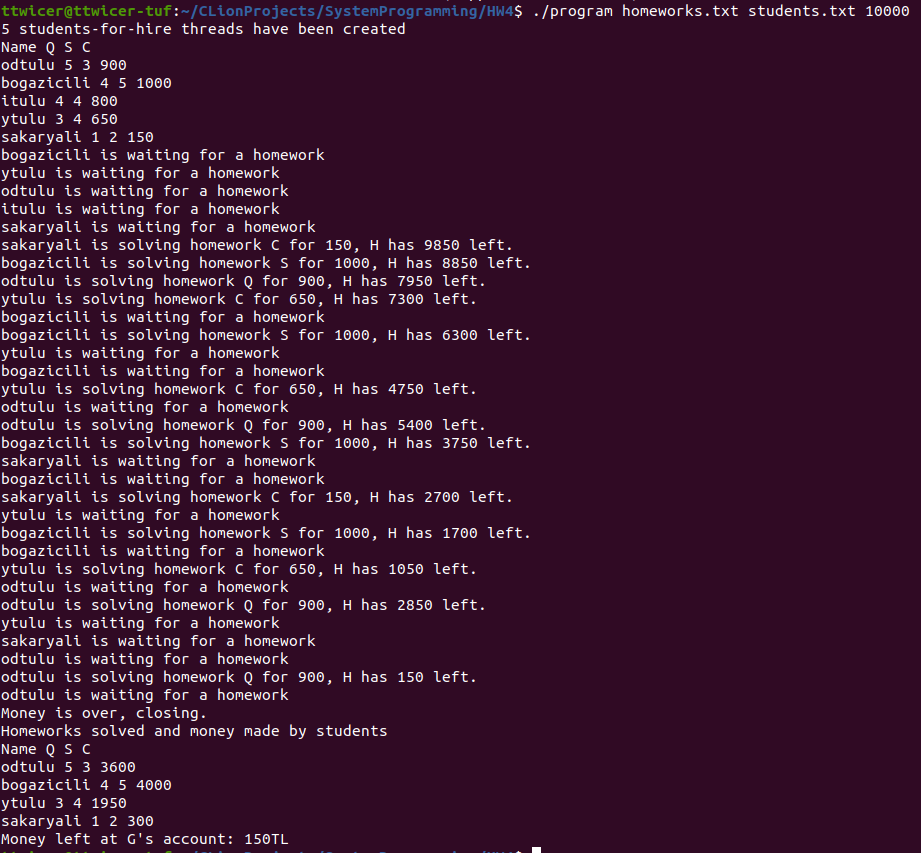
\includegraphics[width=6.55in,height=6.07in]{./image2.png}
	\end{Center}
\end{figure}



\vspace{\baselineskip}
\vspace{\baselineskip}

\vspace{\baselineskip}

\vspace{\baselineskip}

\vspace{\baselineskip}


%%%%%%%%%%%%%%%%%%%% Figure/Image No: 3 starts here %%%%%%%%%%%%%%%%%%%%

\begin{figure}[H]
	\begin{Center}
		
\includegraphics[width=5.0in,height=4.92in]{./image3.png}
	\end{Center}
\end{figure}


%%%%%%%%%%%%%%%%%%%% Figure/Image No: 3 Ends here %%%%%%%%%%%%%%%%%%%%


\vspace{\baselineskip}

%%%%%%%%%%%%%%%%%%%% Figure/Image No: 4 starts here %%%%%%%%%%%%%%%%%%%%

\begin{figure}[H]
	\begin{Center}
		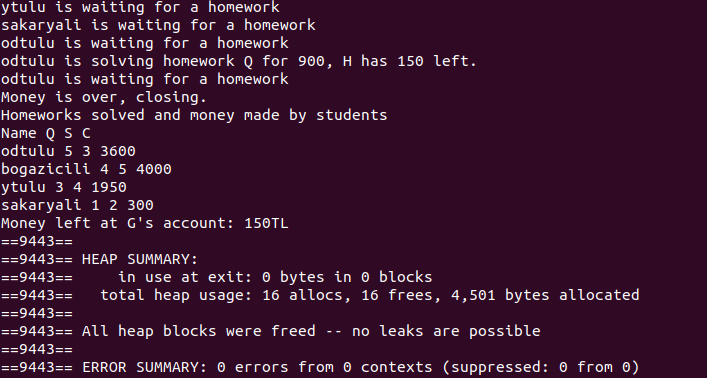
\includegraphics[width=5.0in,height=2.68in]{./image4.png}
	\end{Center}
\end{figure}


%%%%%%%%%%%%%%%%%%%% Figure/Image No: 4 Ends here %%%%%%%%%%%%%%%%%%%%


\vspace{\baselineskip}\printbibliography
\end{document}